\documentclass[a4paper]{scrartcl}
\usepackage[cm]{fullpage}
\usepackage{amsmath, amssymb, esint}
\usepackage{siunitx}
\usepackage[backend = biber, style = numeric-comp]{biblatex}

\usepackage{tikz, pgfplots}
\pgfplotsset{
    compat = 1.12,
    plot/.style = {
        axis lines = middle,
        clip = false
    },
    plot-scatter/.style = {
        only marks,
        error bars/.cd,
        x dir = both, y dir = both,
        x explicit, y explicit
    }
}

\begin{filecontents}{\jobname.bib}
@book{DEL2001,
	author = {P Delhaes},
	title = {Graphite and Precursors},
	date = {2001},
	publisher = {CRC Press},
	isbn = {90-5699-228-7}
}
@misc{linear-regression,
	url = {http://mathematica.stackexchange.com/a/13122},
	year  = {2017},
	month = {mar},
	title = {Estimate error on slope of linear regression given data with associated uncertainty}
}
\end{filecontents}
\addbibresource{\jobname.bib}

\begin{document}

\title{PHYS3112: Electron Diffraction}
\author{ \\ \\ }
\date{2017-03-06}
\maketitle

\section{Abstract}
Powder diffraction of a graphite sample produced plane distances of \SI{1.00 \pm 0.05}{\angstrom} and \SI{1.82 \pm 0.13}{\angstrom}, which are about \SI{19}{\percent} and \SI{15}{\percent} respectively below the expected values of \SI{1.23}{\angstrom} and \SI{2.13}{\angstrom} from the carbon-carbon spacing of \SI{1.42}{\angstrom} found in the literature \cite{DEL2001}.

\section{Materials and Methods}
Please refer to the operating instructions of the experiment and the prework.

The phosphorescent layer was assumed to be on a spherical surface of radius \(R = \SI{64 \pm 3}{\milli\metre}\). In reality, it seemed to be closer to an oblate spheroid with axes lengths \(a = \SI{65 \pm 2}{\milli\metre}\) and \(c = \SI{63 \pm 2}{\milli\metre}\), so this is a reasonable approximation.

The dot at the centre of the rings was assumed to be the true centre, and thus was lined up against when measuring the diameter of the rings. Since the surface is curved, a ruler was placed tangent to this dot, and the diameter measurements ``eyeballed'' to match the markings on the ruler. This effectively gives the diameter as a chord of the surface, though the accuracy is likely no better than \(\pm\SI{1}{\milli\metre}\).

Since the rings are being measured with human eyes, which aren't great at finding maxima in light intensity, the apparent widths of the ring lines were also measured to an accuracy no better than \(\pm\SI{0.5}{\milli\metre}\). These line widths will be accounted for in the rings diameter error.

The diameters and line widths were measured three times, each at different angles. These values were averaged together to provide an overall diameter and error.

We assume \(n = 1\) in the Bragg condition, since we are only considering the brightest rings.

Given the carbon-carbon lattice spacing of graphite as \SI{1.42}{\angstrom}, and assuming the reflection planes as given in the student notes are accurate, we expect the plane separations to be \SI{1.23}{\angstrom} and \SI{2.13}{\angstrom}.

\section{Results}
\begin{table}
    \centering
    \begin{tabular}{c | c | c}
        \(V_{G3}\) (\si{\kilo\volt}) & \(2 r_1\) (\si{\milli\metre}) & \(2 r_2\) (\si{\milli\metre}) \\
        \hline
        \SI{4.0 \pm 0.1}{} & \SI{28 \pm 2}{} & \SI{47 \pm 3}{} \\
        \SI{4.0 \pm 0.1}{} & \SI{27 \pm 2}{} & \SI{46 \pm 3}{} \\
        \SI{4.8 \pm 0.1}{} & \SI{25 \pm 2}{} & \SI{42 \pm 3}{} \\
        \SI{5.4 \pm 0.1}{} & \SI{23 \pm 2}{} & \SI{39 \pm 3}{} \\
        \SI{6.4 \pm 0.1}{} & \SI{21 \pm 1}{} & \SI{37 \pm 3}{} \\
        \SI{7.5 \pm 0.1}{} & \SI{20 \pm 1}{} & \SI{33 \pm 3}{} \\
        \SI{7.5 \pm 0.1}{} & \SI{20 \pm 1}{} & \SI{34 \pm 3}{}
    \end{tabular}
    \caption{Measured diameters}
    \label{tab:diameters}
\end{table}
\begin{figure}
    \centering
    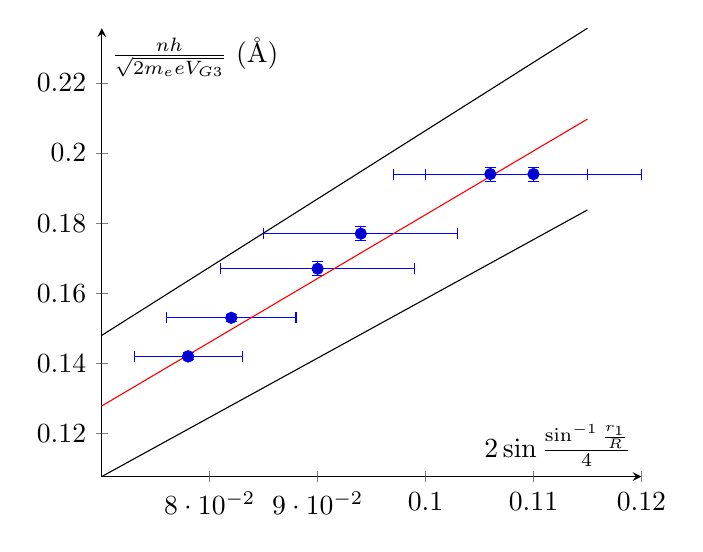
\begin{tikzpicture}
        \begin{axis}[
            plot,
            xlabel = \(2 \sin \frac{\sin^{-1} \frac{r_1}{R}}{4}\),
            ylabel = \(\frac{n h}{\sqrt{2 m_e e V_{G3}}}\) (\si{\angstrom})
        ]
            \addplot +[plot-scatter] table [
                x error = xerror,
                y error = yerror
            ] {
                x       y       xerror  yerror
                0.11	0.194	0.01	0.002
                0.106	0.194	0.009	0.002
                0.094	0.177	0.009	0.002
                0.09	0.167	0.009	0.002
                0.082	0.153	0.006	0.001
                0.078	0.142	0.005	0.001
                0.078	0.142	0.005	0.001
            };
            \addplot +[no marks, domain = 0.07:0.115] {0.000586435 + 1.81822 * x};
            \addplot [no marks, domain = 0.07:0.115] {-0.0105522 + 1.68971 * x};
            \addplot [no marks, domain = 0.07:0.115] {0.0117251 + 1.94672 * x};
        \end{axis}
    \end{tikzpicture}
    \caption{Fit for \(d_1 = \SI{1.82 \pm 0.13}{\angstrom}\)}
    \label{fig:d1-fit}
\end{figure}
\begin{figure}
    \centering
    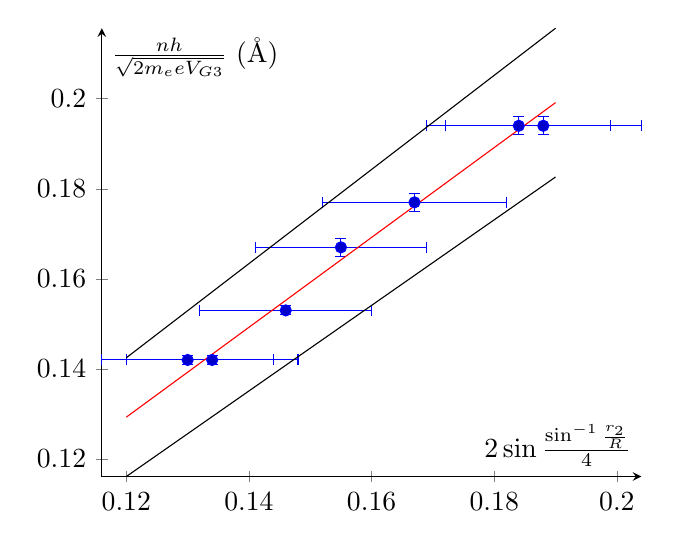
\begin{tikzpicture}
        \begin{axis}[
            plot,
            xlabel = \(2 \sin \frac{\sin^{-1} \frac{r_2}{R}}{4}\),
            ylabel = \(\frac{n h}{\sqrt{2 m_e e V_{G3}}}\) (\si{\angstrom})
        ]
            \addplot +[plot-scatter] table [
                x error = xerror,
                y error = yerror
            ] {
                x       y       xerror  yerror
                0.188	0.194	0.016	0.002
                0.184	0.194	0.015	0.002
                0.167	0.177	0.015	0.002
                0.155	0.167	0.014	0.002
                0.146	0.153	0.014	0.001
                0.13	0.142	0.014	0.001
                0.134	0.142	0.014	0.001
            };
            \addplot +[no marks, domain = 0.12:0.19] {0.00954982 + 0.997867 * x};
            \addplot [no marks, domain = 0.12:0.19] {0.00207845 + 0.950247 * x};
            \addplot [no marks, domain = 0.12:0.19] {0.0170212 + 1.04549 * x};
        \end{axis}
    \end{tikzpicture}
    \caption{Fit for \(d_2 = \SI{1.00 \pm 0.05}{\angstrom}\)}
    \label{fig:d2-fit}
\end{figure}

Table \ref{tab:diameters} shows the measured diameters versus applied voltage after averaging. These were then plotted according to the method outlined in the prework in Figures \ref{fig:d1-fit} and \ref{fig:d2-fit}. A linear regression \cite{linear-regression} was then applied to give estimates on the plane distances, which were \SI{1.00 \pm 0.05}{\angstrom} and \SI{1.82 \pm 0.13}{\angstrom}.

\section{Discussion}
Our measured plane distances of \SI{1.00 \pm 0.05}{\angstrom} and \SI{1.82 \pm 0.13}{\angstrom} are about \SI{19}{\percent} and \SI{15}{\percent} respectively below the expected values of \SI{1.23}{\angstrom} and \SI{2.13}{\angstrom}.

Since it is very unlikely that the values in the literature are incorrect, this is more than likely some kind of systematic error in our experimental setup.

Possible issues could include:
\begin{itemize}
	\item The actual voltage the electrons accelerated through was lower than the applied voltage
	\item The electrons lost energy colliding with the non-perfect vacuum in the chamber
	\item The sample was not placed exactly on the edge of the chamber
	\item The chamber was not spherical like we assumed
\end{itemize}

These could be checked by, respectively:
\begin{itemize}
	\item Check the velocity of the electrons exiting the accelerator and see if it matches our predictions
	\item Vary the vacuum level of the chamber and see how the rings' size changes
	\item Double check the sample position
	\item Use a spherical chamber
\end{itemize}

\section{Conclusion}
\emph{(From abstract)} Powder diffraction of a graphite sample produced plane distances of \SI{1.00 \pm 0.05}{\angstrom} and \SI{1.82 \pm 0.13}{\angstrom}, which are about \SI{19}{\percent} and \SI{15}{\percent} respectively below the expected values of \SI{1.23}{\angstrom} and \SI{2.13}{\angstrom} from the carbon-carbon spacing of \SI{1.42}{\angstrom} found in the literature.

This is more than likely a systematic error in our experimental setup, rather than a groundbreaking discovery.

\printbibliography

\end{document}